% Use only LaTeX2e, calling the article.cls class and 12-point type.

\documentclass[12pt]{article}
\usepackage{bm,url,graphicx} %PJM added these here

% Users of the {thebibliography} environment or BibTeX should use the
% scicite.sty package, downloadable from *Science* at
% www.sciencemag.org/about/authors/prep/TeX_help/ .
% This package should properly format in-text
% reference calls and reference-list numbers.

% Use times if you have the font installed; otherwise, comment out the
% following line.

\usepackage{times}

% The preamble here sets up a lot of new/revised commands and
% environments.  It's annoying, but please do *not* try to strip these
% out into a separate .sty file (which could lead to the loss of some
% information when we convert the file to other formats).  Instead, keep
% them in the preamble of your main LaTeX source file.


% The following parameters seem to provide a reasonable page setup.

\topmargin 0.0cm
\oddsidemargin 0.2cm
\textwidth 16cm
\textheight 21cm
\footskip 1.0cm

% Include your paper's title here

\title{ISE790 Final Project Write-up}

% Place the author information here.  Please hand-code the contact
% information and notecalls; do *not* use \footnote commands.  Let the
% author contact information appear immediately below the author names
% as shown.  We would also prefer that you don't change the type-size
% settings shown here.

\author
{Yuan Zhang and Thomas Richardson}

% Include the date command, but leave its argument blank.

%\date{}



%%%%%%%%%%%%%%%%% END OF PREAMBLE %%%%%%%%%%%%%%%%



\begin{document}

% Double-space the manuscript.

\baselineskip24pt

% Make the title.

\maketitle

\noindent

\section*{Introduction}

Define $\tilde{A}$ as a fuzzy matrix of dimension $m \times n$, $\tilde{x}$ as a fuzzy vector of length $n$ and $\tilde{b}$ a fuzzy vector of length $m$.  We would like to solve $\tilde{A} \circ \tilde{x} = \tilde{b}$.  We may solve

\begin{equation}
(a_{11} \cdot x_1) \vee (a_{12} \cdot x_2) \vee \dots \vee (a_{1n}, x_n) = b_1
\label{eq: first}
\end{equation}

by calculating  $b_1 / a_{1j}$ for each $a_{1j}$ and setting these values as the corresponding $x_j$ values.  For a larger system with multiple rows, we can compute these values for all rows as above, and choose the minimum value from each column as the representative $x_j$ value for column $j$.  This process ensures that $a_{ij} \cdot x_j \leq b_i$ for all $a_{ij}$ as the minimum value for each column is being slescted.  Note that we are not guaranteed a solution even if  $m \geq n$, as a single row may contribute to multiple $x_j$ values, while another row may contribute to none.  That is, the corresponding Eq \ref{eq: first} may be satisfied multiple times for one row, but never satisfied for another.

We can use the above method to solve the problem given in $(3)$ and find the solution $x = [ 0.9 \quad 0.72 \quad 0.81]$.  For this solution, the first row has two satisfying conditions, one for $x_1$ and the other for $x_3$.  We can use this in part $(4)$ of the problem to maximize the function $10x_1 - 5x_2 - 3x_3$ while maintaining the desired equality from $(3)$.  Either $x_1$ or $x_3$ may be modified, but $x_2$ cannot be changed, as it is the only $x$ value that allows row two to satisfy the inequality.  The only choice given the optimization function is to reduce $x_3$ down to $0$.  Therefore, $x =  [ 0.9 \quad 0.72 \quad 0]$.


\section*{Problem 2:  Fuzzy Matrix with Minimization of Squared Differences Problem}

\subsection*{Exact Solution}

For the exact solution, use a non-linear least squares solver (MATLab function, \textit{lsqnonlin}).  The function uses a trust-region-reflective algorithm (TRFA), which can only work when $\tilde{b}$ is at least the size of $\tilde{x}$.  The second method used by the MATLab function does not accept bounds on generated solutions, so there would be no guarantee that the generated solution would be fuzzy.  The trust-region-reflective algorithm uses the concept of trust-regions to approximate the function being optimized.  A simpler function is generated that accurately represents the original function in a small region, referred to as the trust-region.  The algorithm then minimizes the approximation function over the trust-region.  There could potentially be issues with this method, as the least-squares function, $\|\tilde{A}\circ \tilde{x} - \tilde{b}\|^2$, can be non-continuous.  The algorithm also runs the risk of getting caught in a local minimum.  To avoid this, the `help' documentation recommended running the algorithm multiple times, each time starting from the previously obtained solution.

As we see below, this method does not provide an exact solution to the problem at hand, but it does provide a reasonable function to compare the GA against, as it is designed for optimizing non-linear problems involving minimization of squared differences.

\subsection*{GA Soft-Computing Solution}

The proposed soft-computing approximate solution method is a genetic algorithm with pre-processing to reduce the potential $x_i$ values to sets of discrete cases, $s_i$, determined by values in $A$ and $b$, where $A$ is an $m$-by-$n$ matrix, $b$ is a vector of length $m$, and $x$ is a vector of length $n$.  Initially, each $s_i$ is started $A_{:i}$.  If all values in this vector are larger than the minimum $b$ value, it is added to the list.  The midpoints of this sorted vector are then added, and the resulting sorted vector is the initial $s_i$.  The maximum size of each $s_i$, then, is $2*m+1$.  Each $x_i$ domain is not necessarily fixed for the entirety of the algorithm's progression; the set of possible values for each $x_i$ may be updated after some set number of iterations if the values present in the population have converged to some smaller sub-set of values than the original $s_i$.  This allows the algorithm to explore various resolutions of solutions.  

Discretizing the domain of $x$ allows for a simple chromosome encoding; each chromosome is represented by a vector of integers $c$, where each entry $c_i$ of $c$ corresponds to a particular member of $s_i$ such that $c_i \in \{1, \dots, | s_i |\}$ and each $x_i$ has a representative $c_{\{i\}}$ in $c$.  This encoding allows for easy manipulation, storage, and updating of chromosomes; all chromosomes can be stored in a matrix $C$, where each column of $C$ is a chromosome $c$.  Additionally, the basic rules and tools for genetic algorithms can be employed on chromosomes of this type.

The population size is fixed at a size determined by the size of the solution space, where $| Solution Space | = \prod_{i=1}^{n} | s_i |$.  Specifically, $PopSize = k*| Solution Space |$, where $1 \leq k \leq 2$.  To maintain a constant population size, after new solutions are generated, only the best $PopSize$ solutions remain in the population.  Duplicate solutions are allowed in the population.

The solution population is updated using a combination of two tools:  recombination and mutation.  At each iteration, $PopSize$ new solutions are generated from the starting population.  Recombination is performed by combining elements from some number of parents from the starting population, and can be single point or multi-point.  The algorithm employed uses multi-point, multi-point recombination, with $p \in \{2,4,5,8\}$ parents \cite{vasko} and each gene for the chromosome being selected independently.  To create a new offspring chromosome, a parent number, $p$, is selected in a weighted-random fashion (more on that later), as well as $p$ chromosomes from the current population (excluding any newly generated chromosomes from the current iteration; also, recent picks are also Tabued from being used again).  A pseudo-random matrix is created in MATLab with $n$ rows and $p$ columns such that a one-to-one mapping exists between selected parent chromosomes and columns in the generated matrix.  Each column in this matrix is then multiplied by the score value of the corresponding parent chromosome, where a score value is a measure of the fitness of a particular chromosome.  The maximum value for each row is then found, and the gene from the corresponding chromosome is used as the gene for the offspring.  The mean gene value is used if a tie ensues between multiple parents.  

A mutation is attempted following the creation of offspring via crossover.  If the mean score of the parents is less than the mean population score, a mutation is always performed.  Otherwise, a mutation is performed with probability $e^{-\frac{mean(parents-scores)}{mean(population-scores)}}$.  A random gene and gene value are selected for mutation.  This restricts movement away from what should be `better' solutions while allowing what should be  `worse' solutions to mutate.

After the new set of chromosomes is constructed, the fitness values and corresponding scores are calculated for each new chromosome.  Note that these are two different values.  The fitness is the particular value obtained by evaluating the objective function with a given solution represented by a chromosome; chromosomes are not solutions in themselves, but map to solutions.  In this case, the fitness of a chromosome is calculated by $\|A\circ x - b\|^2$.  The score for a particular chromosome is a value calculated from the fitness value, and is typically a function of all fitness values from the population.  Two score functions were utilized for this problem, an exponential-based score function, and a linear-based score function, calculated by $s_i = \frac{e^{-fitness_i}}{\sum_{j}^{PopSize}e^{-fitness_j}}$ and $s_i = \frac{fitness_i}{\sum_{j}^{PopSize}fitness_j}$, respectively.  The former can be used early on to quickly converge to a set of `good' solutions, while the latter can be used at later stages to allow fine-tuning of the population to a `best' solution or solutions.

There are several options for terminating the algorithm.  One is simply allowing the algorithm to run for some pre-determined number of iterations, at the end of which the best solution is presented as the problem solution.  Another method is halting after some consecutive number of iterations fail to result in a change in the best fitness score found, or if some minimal improvement is not made.  A third would to be halt once the current population becomes dominated by a single solution or some small subset of solutions.

\subsection{Examples}

The only reasonable example I could come up with was a fuzzy random matrix $A$ and a corresponding fuzzy random vector $b$.  As the pseudo-random typically lack any underlying patterns, attempting to minimize the function $\|A\circ x - b\|^2$ should be taxing on the algorithms.   Several instances were run for various sized $A$ matrices, but always with the number of rows greater than or equal to the number of columns, as this is the only region for which the `exact' algorithm operates.  The results show that the MATLab algorithm does not find an exact solution to the problem at hand, as the GA constructed for this problem outperformed it on several occasions.  As noted above, this could potentially have something to do with the function being dis-continious.  The TRFA did perform faster in all cases, and significantly faster for the largest graph tested (see Fig \ref{fig: FMCompare}, note the $log$ scale for time).  However, the TRFA underperformed the GA for larger graph sizes in finding a minimum $x$ vector.  The GA could still use some improvement time-wise, though.  One particular option would be removing the Tabued parenthood, so that a larger portion of the offspring generated in each iteration were from the best previous members of the population, thereby potentially converging to an optimal solution in fewer iterations.  Another way to reduce runtime may be to decrease the number of possible $x$ values, thereby decreasing the domain, allowing for a smaller solution population (though the domain of $x$ could be reduced independently of reducing the solution space if desired).


%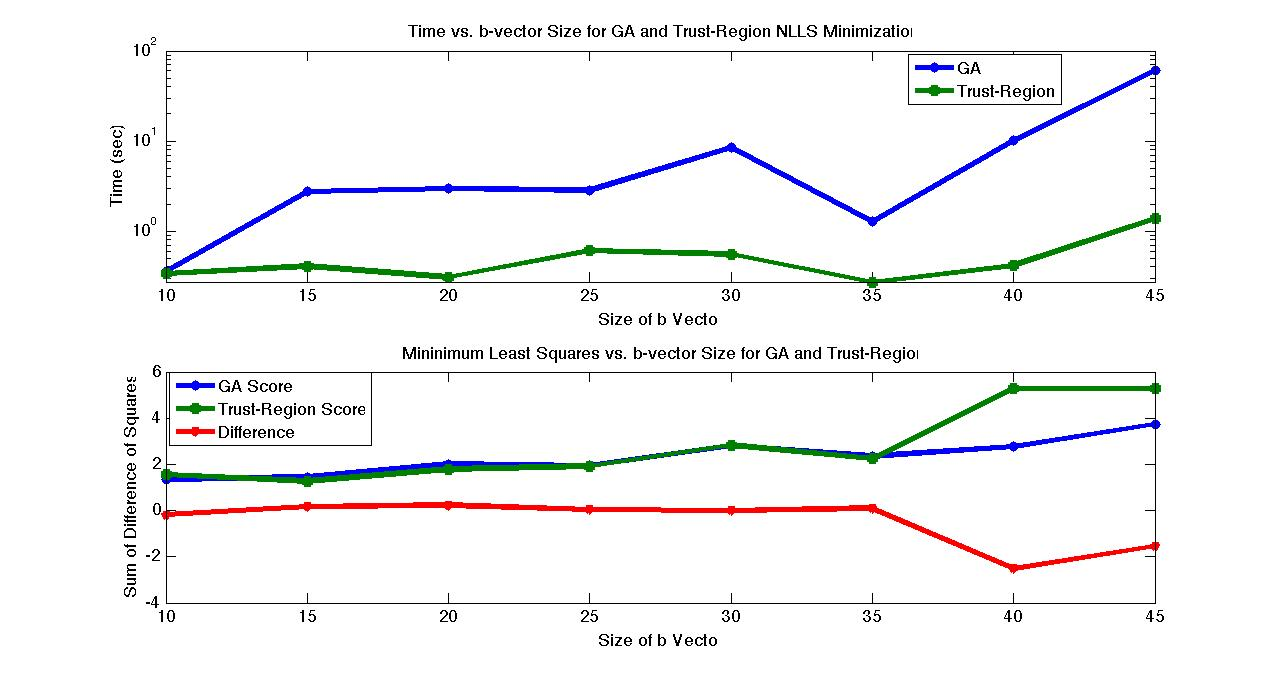
\includegraphics[width=1.1\textheight, angle = -90]{ComparisonPlotFM.jpg}
%\caption{Comparison of Results for Max Cut Problem for Tabu Search and Exact Algorithms}
%\label{fig: FMCompare}


\section*{Problem 3:  Max Cut Problem}

\subsection*{Exact Solution}

A simple approach to solving the Max Cut problem exactly involves encoding the solution as $x = \{0,1\}^n$, where $n$ is the number of vertices in the graph, and each entry represents whether the corresponding vertex is in one partition or the other, as the max cut problem partitions the graph into two groups.  Since $x$ has only binary values, and since each solution vector has a complement solution vector for which the sum of the solutions is $2^n$, the size of the solution space is $2^{n-1}$, so any intuitive algorithm to determine the solution runs in super-polynomial time with complexity $O(2^{n-1})$.  The graph cut decision problem is in $NP$, but it would not seem that checking whether a proposed cut is the max cut cannot be checked in polynomial time unless the max cut problem is in $P$.

\subsection*{Tabu-Search Soft-Computing Solution}

A Tabu-based search is an effective soft-computing method to find the max cut of a graph.  The principle idea of Tabu search is that decisions made in the recent past are not repeated or undone.  This can force an algorithm to switch to proposed solutions that are worse than a previously found solution, allowing the algorithm to burrow out of local minima.  To prevent permanently moving away from an optimal solution, the best solution found thus far is stored in memory.   

For this problem, the algorithm moves through solutions by considering a subset of neighbors, $S$, for the current solution $C$, and computes the quality score for each of these neighbors.  If the neighbor in $S$ with the best quality score was not obtained by a move in the Tabu list, $T$, then it becomes the new current solution, $C '$, regardless of whether its quality score is better or worse than the starting proposed solution for the current iteration.  If the best neighbor is arrived at via a move in $T$, then it becomes $C '$ only if its quality score is strictly greater than the best quality score found so far by the algorithm (aspiration criteria).  If this is not the case, then all neighbors in $S$ that are obtained by a move in $T$ are removed from consideration, and the remaining best neighbor is selected as $C �$.  Various checks are in place to deal with situations where all neighbors in $S$ correspond to moves in $T$.  In any case, the move corresponding to the transition from $C$ to $C �$ is placed in $T$ for the pre-set tenure period; if it was already in $T$, then its remaining time in $T$ is reset to the tenure period.  For the particular instance of Tabu search used, the tenure period is set to $\frac{N}{3}$, where $N$ is the number of vertices in the graph.  Several values were tried, and this seemed to work best.

Encoding solutions for the Tabu algorithm is the same as for the exact case, a binary vector of length $n$.  The neighbors of $C$ are then defined as all vectors $N$ that can be obtained by flipping a single bit in $C$.  Therefore, each $C$ has a rather small number of neighbors, $n$, in comparison to the size of the search space.  Using a single flip as a neighbor instead of multiple flips makes encoding and transitioning rather simple, while also minimizing the number of neighbors for a given solution, thereby minimizing the potential number of solutions to consider at each iteration.  The initial solution is created pseudo-randomly using the MATLab \textit{rand} function.  Modifications in creating this starting solution could be made if something was known about the adjacency matrix for the graph being analyzed.  Iterations of the algorithm are performed until there is no change in the best-found solution for $N$ consecutive steps.  There is no upper-bound on the number of total iterations, and the algorithm has not yet failed to terminate.

An additional performance feature for the Tabu search is to run the algorithm multiple times from a new, random starting point each time.  The best solution obtained from each run is recorded and compared to the best run from all other runs, with the best overall solution being taken as the output for the algorithm.

\subsection*{Examples}

A useful example to compare the performance of the exact and Tabu algorithms is the adjacency matrix, $A$, from HW6, where $A_{ij}$ is calculated as $\frac{i^2 + j^2}{i + j}$.  The two algorithms can be compared for relatively small matrices, as the algorithm calculating the exact solution beings to become intolerably slow around $N = 20$.  Fig \ref{fig: TabuCompare} shows the run times and resulting scores from a small  set of graphs.  The plots verify the accuracy and speed of the Tabu method, at least on small graphs, in comparison to the exact method.  In the second plot there appear to be only two lines because the scores corresponding to the Exact Algorithm and the Tabu Search are nearly indistinguishable.


\clearpage

\begin{thebibliography}{9}
 
\bibitem{vasko}
  FJ Vaskol, PJ Knolle and DS Spiegel, 
  \textit{JSTOR} \textbf{56}, 10 (2005), pp.1213-1223
  

  
 
\end{thebibliography}



\end{document}




